\documentclass[12pt,a4paper]{article}
\usepackage[utf8]{inputenc}
\usepackage[spanish]{babel}
\usepackage{amsmath}
\usepackage{amsfonts}
\usepackage{amssymb}
\usepackage{graphicx}
\usepackage{kpfonts}
\usepackage[left=2cm,right=2cm,top=2cm,bottom=2cm]{geometry}
\title{EV 1-6 OPERACIÓN DE CIRCUITOS DE ACTIVACIÓN CON TIRISTORES EN CONVERTIDORES DE CA-CD y CA-CA

\includegraphics [scale=1]{imagenes/UPZMG.png} 
\author{Alan Antonio Muñoz Juarez\\
\small Sistemas electrónicos de interfaz\\
  \small Universidad Politécnica de la zona metropolitana de Guadalajara\\
  \small 4°B \\
  \small Ing. Mecatrónica\\
\centering
\linebreak
}
}

\begin{document}
\maketitle
\newpage
\begin{flushleft}
\section {¿Cuales son los los amplificadores clase A?}
\end{flushleft}
Los amplificadores clase A son aquellos amplificadores cuyas etapas de potencia consumen corrientes altas y continuas de su fuente de alimentación, independientemente de si existe señal de audio o no.\\
La función principal del amplificador de potencia, que también se conoce como amplificador de señal grande, es suministrar potencia, que es el producto del voltaje y la corriente de la carga. Básicamente, un amplificador de potencia también es un amplificador de tensión, con la diferencia de que la resistencia de carga conectada a la salida es relativamente baja.
\begin{center}
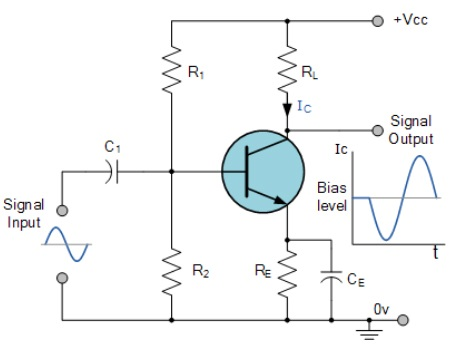
\includegraphics[scale=1]{imagenes/amplificadorA.JPG} 
\end{center}
\subsection{Características principales}
\begin{flushleft}
Esta amplificación presenta el inconveniente de generar una fuerte y constante emisión de calor. No obstante, los transistores de salida están siempre a una temperatura fija y sin alteraciones.\linebreak

En general, se afirma que esta clase de amplificación es frecuente en circuitos de audio y en los equipos domésticos de gama alta, ya que proporcionan una calidad de sonido potente y de muy buena calidad.\linebreak

Los amplificador de clase A a menudo consisten en un transistor de salida conectado al positivo de la fuente de alimentación y un transistor de corriente constante conectado de la salida al negativo de la fuente de alimentación.\linebreak

La señal del transistor de salida modula tanto el voltaje como la corriente de salida. Cuando no hay señal de entrada, la corriente de polarización constante fluye directamente del positivo de la fuente de alimentación al negativo, resultando que no hay corriente de salida, se gasta mucha corriente. Algunos amplificador de clase A más sofisticados tienen dos transistores de salida en configuración push-pull.\newpage
\end{flushleft}
\begin{center}
\section {Arreglos en amplificadores clase A}
\end{center}
El amplificador de Clase A es la forma más simple de amplificador de potencia que utiliza un solo transistor de conmutación en la configuración de circuito de emisor común estándar como se ha visto anteriormente para producir una salida invertida. El transistor siempre está polarizado en "ON" para que conduzca durante un ciclo completo de la forma de onda de la señal de entrada, produciendo la mínima distorsión y la máxima amplitud de la señal de salida.\linebreak
Esto significa que la configuración del amplificador de clase A es el modo de funcionamiento ideal, ya que no puede haber distorsión de cruce o desconexión a la forma de onda de salida incluso durante la mitad negativa del ciclo. Las etapas de salida del amplificador de potencia de Clase A pueden usar un único transistor de potencia o pares de transistores conectados entre sí para compartir la corriente de alta carga. Considere el circuito amplificador Clase A a continuación.\\


\subsection{Circuito amplificador de una sola etapa}
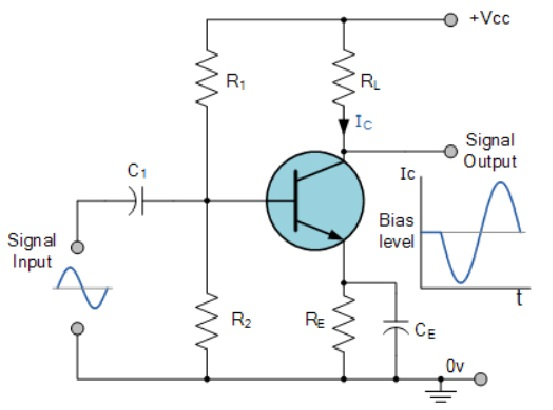
\includegraphics[scale=.8]{imagenes/1ETAPA.JPG} 
\begin{flushleft}
Este es el tipo más simple de circuito amplificador de potencia Clase A. Utiliza un transistor de extremo único para su etapa de salida con la carga resistiva conectada directamente al terminal colector. Cuando el transistor se "enciende", se hunde la corriente de salida a través del Colector, lo que resulta en una caída de voltaje inevitable a través de la resistencia del Emisor, limitando así la capacidad de salida negativa.\linebreak

La eficiencia de este tipo de circuito es muy baja (menos del 30 por ciento) y ofrece pequeñas salidas de potencia para un gran drenaje en la fuente de alimentación de CC. Una etapa de amplificador de Clase A pasa la misma corriente de carga incluso cuando no se aplica señal de entrada, por lo que se necesitan disipadores de calor grandes para los transistores de salida.\\
\end{flushleft}
\newpage
\begin{flushleft}
\subsection{Circuito amplificador acoplado a transformador}
Como la corriente del colector, Ic se reduce por debajo del punto Q quieto establecido por la tensión de polarización básica, debido a las variaciones en la corriente base, el flujo magnético en el núcleo del transformador se colapsa causando una fem inducida en los devanados primarios del transformador. \\
Esto hace que una tensión instantánea del colector aumente a un valor del doble de la tensión de alimentación de 2 Vcc, lo que da una corriente de colector máxima de dos veces Ic cuando el voltaje del colector está en su mínimo. Entonces la eficiencia de este tipo de configuración del amplificador de clase A se puede calcular de la siguiente manera: 
\end{flushleft}
\begin{center}
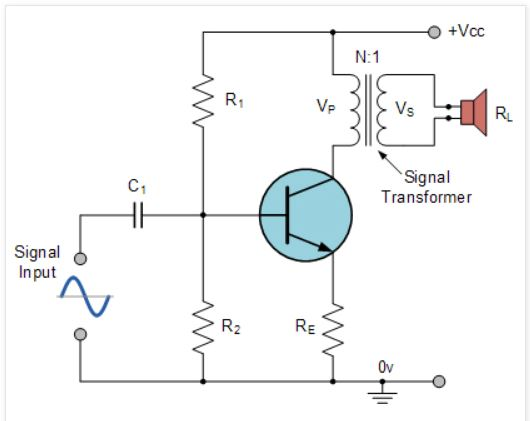
\includegraphics[scale=1.2]{imagenes/transformador.JPG}
\end{center}
\newpage 
\begin{center}
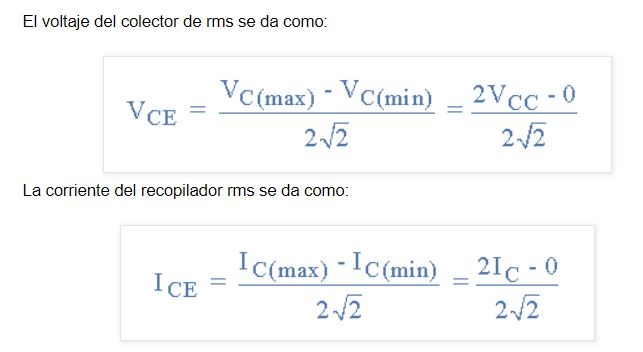
\includegraphics[scale=0.8]{imagenes/calculos.JPG}
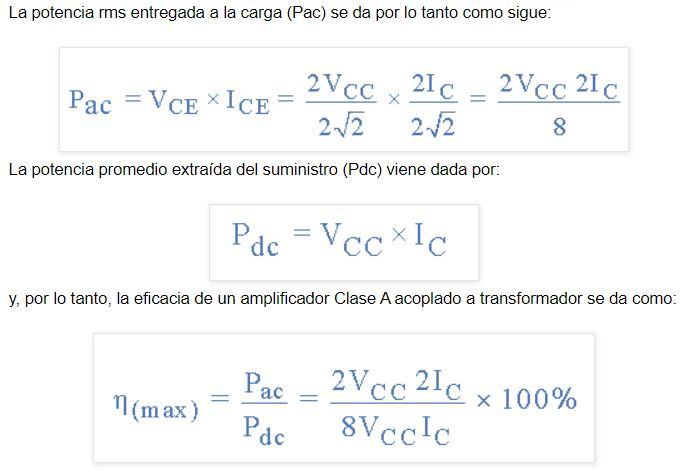
\includegraphics[scale=0.8]{imagenes/calculos1.JPG} 
\end{center}
Un transformador de salida mejora la eficiencia del amplificador al hacer coincidir la impedancia de la carga con la de la impedancia de salida del amplificador. Al utilizar un transformador de salida o de señal con una relación de espiras adecuada, las eficiencias del amplificador de clase A que alcanzan el 40 por ciento son posibles con la mayoría de los amplificadores de potencia de clase A disponibles en este tipo de configuración.\linebreak

Es posible obtener una mayor potencia de salida y eficiencia que la del amplificador de clase A mediante el uso de dos transistores complementarios en la etapa de salida con un transistor de tipo NPN o N-channel, mientras que el otro transistor es un PNP o P-channel (el complemento) tipo conectado en lo que se llama una configuración "push-pull".\\
\newpage
\section{Parámetros en amplificadores clase A}
\begin{flushleft}
Una de las principales desventajas de los amplificadores de potencia y especialmente del amplificador de Clase A es que su eficiencia de conversión general es muy baja ya que las grandes corrientes significan que se pierde una cantidad considerable de energía en forma de calor. La eficiencia porcentual en los amplificadores se define como la potencia de salida rms disipada en la carga dividida por la potencia total de CC tomada de la fuente de suministro como se muestra a continuación.\linebreak
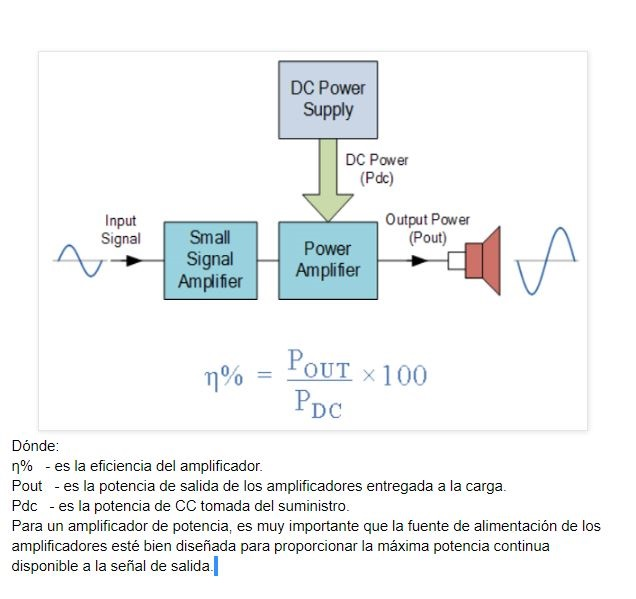
\includegraphics[scale=1]{imagenes/parametros.JPG} 
\newpage
\begin{flushleft}
\section{Referencias bibliográficas}
Javier S.. (2014). Amplificadores de potencia. 01/10/19, de unicrom Sitio web: https://unicrom.com/amplificadores-de-potencia-clasificacion/
\linebreak
\linebreak
Eduardo R.. (2015). El amplificador clase A. 01/10/19, de Blogger Sitio web: http://tutorialesdeelectronicabasica.blogspot.com/2018/06/el-amplificador-de-clase-es-un.html
\linebreak
\linebreak
Angel R.. (2016). amplificadores clase A. 01/10/19, de wordpress Sitio web: https://electronicavm.files.wordpress.com/2011/03/amplificadores-clase-a-y-b1.pdf
\end{flushleft}
\end{flushleft}
\end{document}

\section{se}